\subsection{Vitesse et vecteur vitesse}
Une trajectoire ne suffit pas pour déterminer le mouvement d'un point dans un repère. En effet, cette trajectoire peut-être faite de manière rapide ou lente. La rapidité ou la lenteur est représentée par la vitesse du point.

\UPSTIaRetenir{
La vitesse d'un point est représentée par
\begin{itemize}
  \item de direction tangente à la trajectoire du UPSTIpointilles
  \item de même sens que la trajectoire du point
  \item de norme égale au déplacement divisé par la durée du déplacement
\end{itemize}

  La vitesse moyenne d'un point $M$ se déplaçant de $M(t_1)$ à $M(t_2)$ est de \UPSTIcadreMath{\norme{\vVitesse{M}{}{}} = \frac{M(t_1)M(t_2)}{t_2-t_1}}.

  En écrivant $d$ la distance $d = M(t_1)M(t_2)$ et avec $\Delta t = t_2-t_1$, on a \UPSTIcadreMath{\norme{\vVitesse{M}{}{}} = \frac{M(t_1)M(t_2)}{t_2-t_1} =  \huge{\frac{d}{\Delta t}}}

  La vitesse s'exprime en \si{m/s}.
}

\begin{figure}
  \centering
  \begin{tikzpicture}
  \path(0 ,0)coordinate(A);
  \path(3 ,3)coordinate(B);
  \path(8 ,0)coordinate(C);
  \path(1 ,1)coordinate(ctrl1);
  \path(0 ,3)coordinate(ctrl2);
  \path(6 ,3)coordinate(ctrl3);
  \path(6 ,0)coordinate(ctrl4);
  \draw(A)  .. controls(ctrl1)and(ctrl2)  ..  (B) .. controls(ctrl3)and(ctrl4) .. (C);%
  \draw[->,red,very thick] (B) -- (ctrl3) node[near end, above] {\vVitesse{B}{}{0}};;
  \draw[red] (B) node{$\bullet$} node[above]{B};
  \draw[->,blue,very thick] (A) -- (ctrl1) node[near end, below right] {\vVitesse{A}{}{0}};
  \draw[blue] (A) node{$\bullet$} node[below]{A};
\end{tikzpicture}

  \caption{La vitesse d'un point est tangeante à la trajectoire}
  \label{fig:exemple}
\end{figure}

\UPSTIattention{La vitesse d'un point est un \textbf{vecteur}. Elle a donc une composante sur \vx{}, sur\vy{} et sur \vz{}.}


\begin{UPSTIactivite}
  \begin{center}
    \begin{tikzpicture}
  \draw [very thin, gray] (0,0) grid (12,6);
  \path(0 ,0)coordinate(A);
  \path(3 ,2)coordinate(B);
  \path(10 ,4)coordinate(C);
  \path(0 ,2)coordinate(ctrl1);
  \path(2 ,1)coordinate(ctrl2);
  \path(4 ,3)coordinate(ctrl3);
  \path(10 ,2)coordinate(ctrl4);
  \path(10, 6)coordinate(ctrl5);
  \draw(A)  .. controls(ctrl1)and(ctrl2)  ..  (B) .. controls(ctrl3)and(ctrl4) .. (C);%
  \UPSTIprofOnly{\draw[->,red,very thick] (B) -- (ctrl3) node[near end, above left] {\vVitesse{B}{}{0}};}
  \draw[red] (B) node{$\bullet$} node[above]{B};
  \UPSTIprofOnly{\draw[->,blue,very thick] (A) -- (ctrl1) node[near end, right] {\vVitesse{A}{}{0}};}
  \draw[blue] (A) node{$\bullet$} node[below]{A};
  \UPSTIprofOnly{\draw[->,darkspringgreen,very thick] (C) -- (ctrl5) node[near end, right] {\vVitesse{C}{}{0}};}
  \draw[darkspringgreen] (C) node{$\bullet$} node[right]{C};
\end{tikzpicture}

  \end{center}
  \UPSTIquestion{Tracer l'allure des vecteurs vitesses des points A, B et C}
\end{UPSTIactivite}


\subsection{Accélération - Variation de vitesse}
Nous venons de voir que la vitesse moyenne représente la variation de la position sur un intervalle de temps. De la même façon, l'accélération modélise la variation de vitesse sur un intervalle de temps.

\UPSTIaRetenir{
L'accélération correspond à la variation de vitesse entre deux instants :
\UPSTIcadreMath{a = \frac{v(t_2)-v(t_1)}{t_2-t_1}=\frac{\Delta v}{\Delta t}}, avec $v(t_i)$ la norme de la vitesse à l'instant $t_i$.

L'accélération s'exprime en $m/s^2$.
}

\UPSTIaRetenir{
Lorsque la vitesse est constante, l'accélération est nulle.
}

\begin{UPSTIactivite}
  \resetNumQuestion
  \begin{center}
    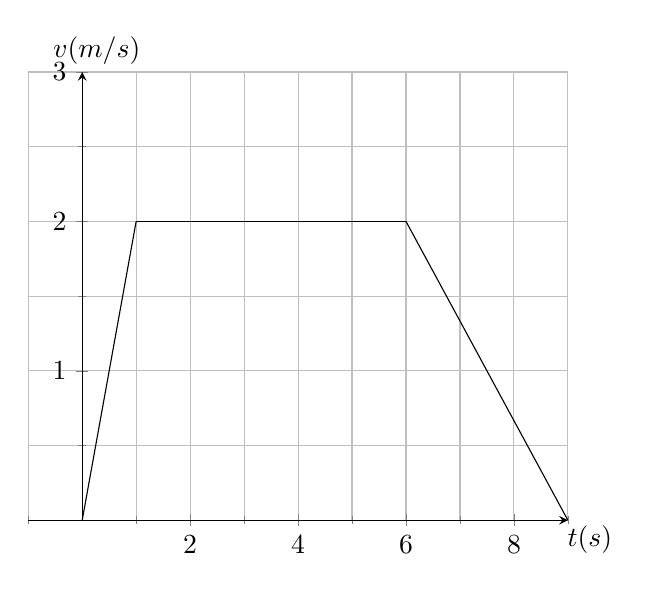
\begin{tikzpicture}
  \begin{axis}[grid=both,%
    %axis x line=center,%
  %axis y line=center,%
    ymin=0,ymax=3,xmax=9,xmin=-1,%
    %xticklabel=\empty,%
    %yticklabel=\empty, %
    minor tick num=1,axis lines = middle,xlabel=$t(\si{s})$,ylabel=$v(\si{m/s})$,label style =
               {at={(ticklabel cs:1.1)}}]
    \addplot [mark=none,domain=0:1] {2*x};
    \addplot [mark=none,domain=1:6] {2};
    \addplot [mark=none,domain=6:9] {6 -2*x/3};
  \end{axis}
  % \draw [very thin, gray] (0,0) grid (12,4);
  % \path(0 ,0)coordinate(A);
  % \path(3 ,2)coordinate(B);
  % \path(10 ,4)coordinate(C);
  % \path(0 ,2)coordinate(ctrl1);
  % \path(2 ,1)coordinate(ctrl2);
  % \path(4 ,3)coordinate(ctrl3);
  % \path(10 ,2)coordinate(ctrl4);
  % \path(10, 6)coordinate(ctrl5);
  % \draw(A)  .. controls(ctrl1)and(ctrl2)  ..  (B) .. controls(ctrl3)and(ctrl4) .. (C);%
  % \UPSTIprofOnly{\draw[->,red,very thick] (B) -- (ctrl3) node[near end, above] {\vVitesse{B}{}{0}};}
  % \draw[red] (B) node{$\bullet$} node[above]{B};
  % \UPSTIprofOnly{\draw[->,blue,very thick] (A) -- (ctrl1) node[near end, below right] {\vVitesse{A}{}{0}};}
  % \draw[blue] (A) node{$\bullet$} node[below]{A};
  % \UPSTIprofOnly{\draw[->,blue,very thick] (C) -- (ctrl5) node[near end, below right] {\vVitesse{C}{}{0}};}
  % \draw[darkspringgreen] (C) node{$\bullet$} node[right]{C};
\end{tikzpicture}

  \end{center}

  \UPSTIquestion{Sur le graph, identifier trois phase de mouvement différentes.}

  \UPSTIquestion{Calculer l'accélération moyenne entre $t=\SI{0}{s}$ et $t=\SI{1}{s}$. }

  \UPSTIeleveOnly{\UPSTIpointilles}

  \UPSTIcorrection{$a=\frac{\Delta v}{\Delta t} = \frac{2}{1} = \SI{2}{m/s^2}$}

  \UPSTIquestion{Calculer l'accélération moyenne entre $t=\SI{1}{s}$ et $t=\SI{6}{s}$. }

  \UPSTIeleveOnly{\UPSTIpointilles}

  \UPSTIcorrection{$a=\frac{\Delta v}{\Delta t} = \frac{0}{1} = \SI{0}{m/s^2}$}

  \UPSTIquestion{Calculer l'accélération moyenne entre $t=\SI{6}{s}$ et $t=\SI{9}{s}$. }

  \UPSTIeleveOnly{\UPSTIpointilles}

  \UPSTIcorrection{$a=\frac{\Delta v}{\Delta t} = \frac{2}{3} = \SI{-0,66}{m/s^2}$}
  \resetNumQuestion
\end{UPSTIactivite}
